%======================================================================
\chapter{Numerical Simulations}
%\chapter{MATLAB Simulations}
\label{ch: Chapter4}
%======================================================================

%----------------------------------------------------------------------
\section{LQR (P controller)}
%----------------------------------------------------------------------
Using MATLAB, we created a program, as seen in \ref{ch:codeLQRsim}, that calculates LQR for our helicopter and then uses differential equations to simulate the trajectory. \ref{fig:LQR_Pos_Con} \ref{fig:LQR_Error_Con}  \ref{fig:LQR_Volt_Con}  

\begin{figure}[!htbp]
    \centering
    \subfigure[][]{
    %\missingfigure{Insert figure.}
    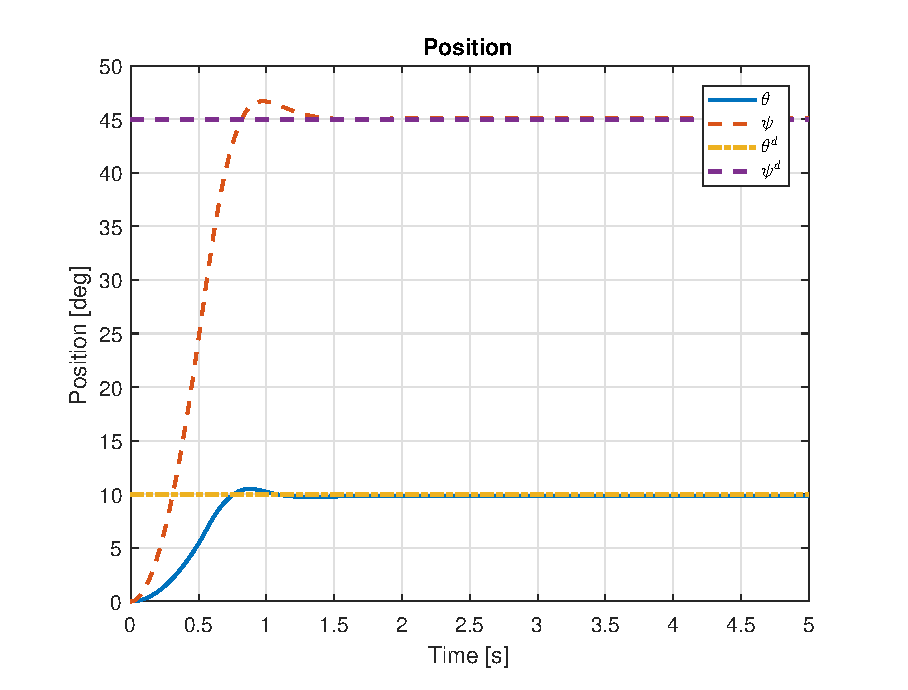
\includegraphics[width=.46\textwidth,keepaspectratio=true]{figs/matlab/LQR/P_Simulation/LQR_Pos_Con.eps}
    \label{fig:LQR_Pos_Con}
    }
    \subfigure[][]{
    %\missingfigure{Insert figure.}
    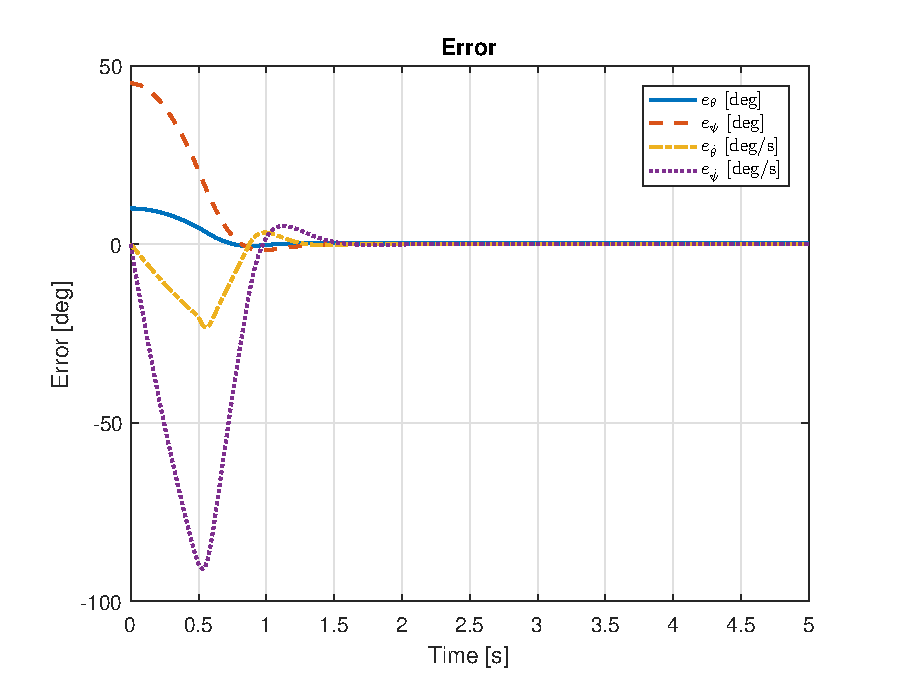
\includegraphics[width=.46\textwidth,keepaspectratio=true]{figs/matlab/LQR/P_Simulation/LQR_Error_Con.eps}
    \label{fig:LQR_Error_Con}
    }
    \subfigure[][]{
    %\missingfigure{Insert figure.}
    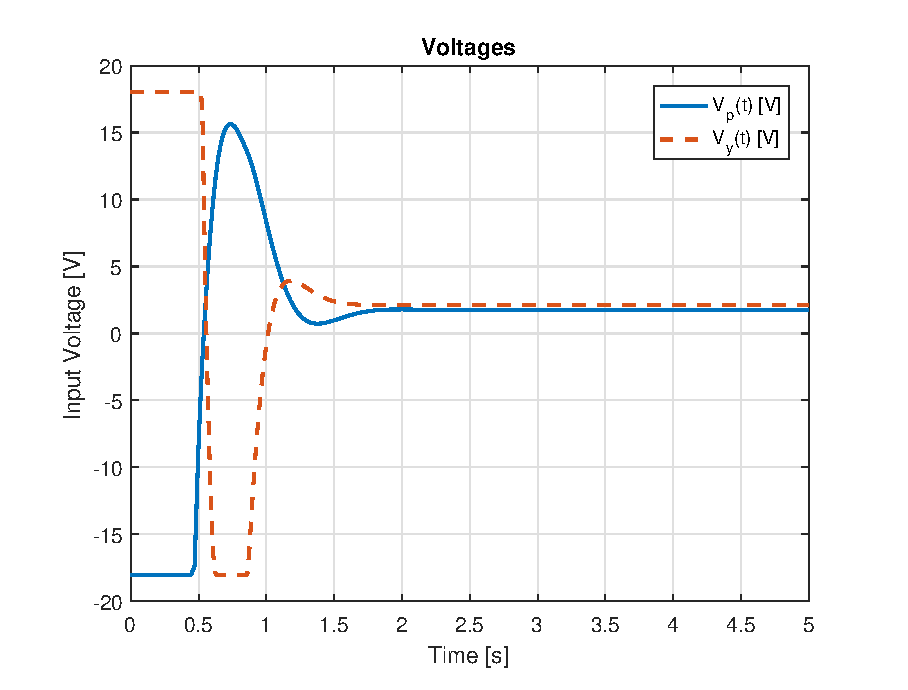
\includegraphics[width=.46\textwidth,keepaspectratio=true]{figs/matlab/LQR/P_Simulation/LQR_Volt_Con.eps}
    \label{fig:LQR_Volt_Con}
    }
    \caption{Simulations for proportional gain calculated by LQR.}
\end{figure}

%----------------------------------------------------------------------
\section{LQR (PI controller)}
%----------------------------------------------------------------------
\todo[inline]{Insert Block diagram for LQR PI simulation}
%\todo[inline]{Insert results for LQR PI simulation}
\begin{figure}[!htbp]
    \centering
    \subfigure[][]{
    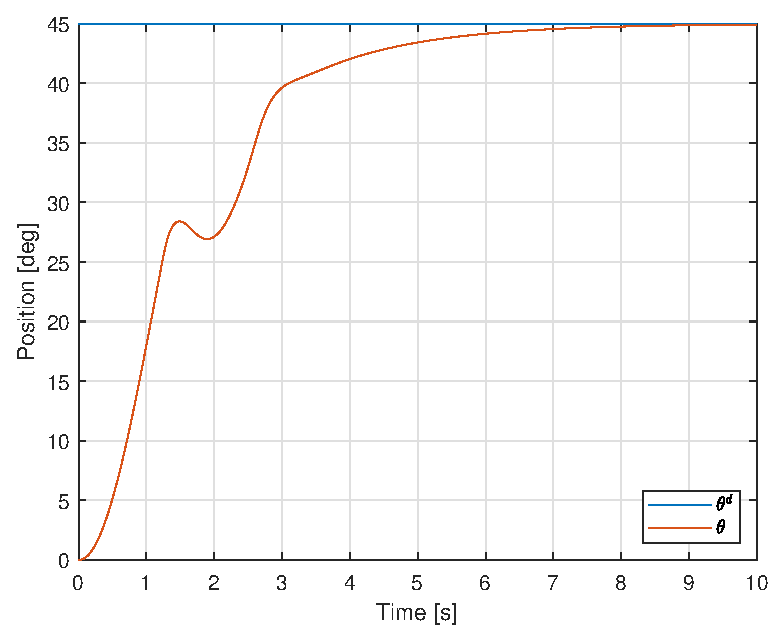
\includegraphics[width=.46\textwidth,keepaspectratio=true]{figs/matlab/LQR/PI_Sim/Pitch_LQR_Sim.eps}
    \label{fig:Pitch_LQR_Sim}
    }
    \subfigure[][]{
    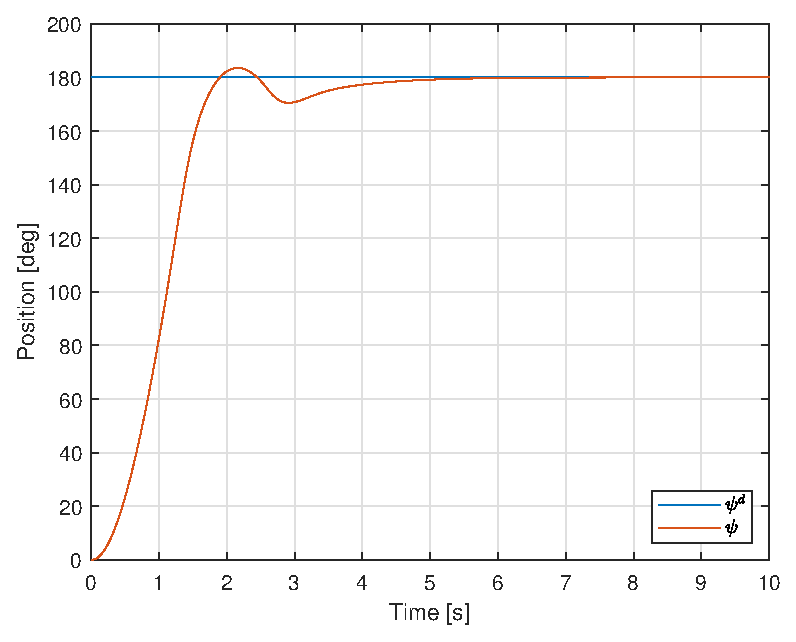
\includegraphics[width=.46\textwidth,keepaspectratio=true]{figs/matlab/LQR/PI_Sim/Yaw_LQR_Sim.eps}
    \label{fig:Yaw_LQR_Sim}
    }    
    \subfigure[][]{
    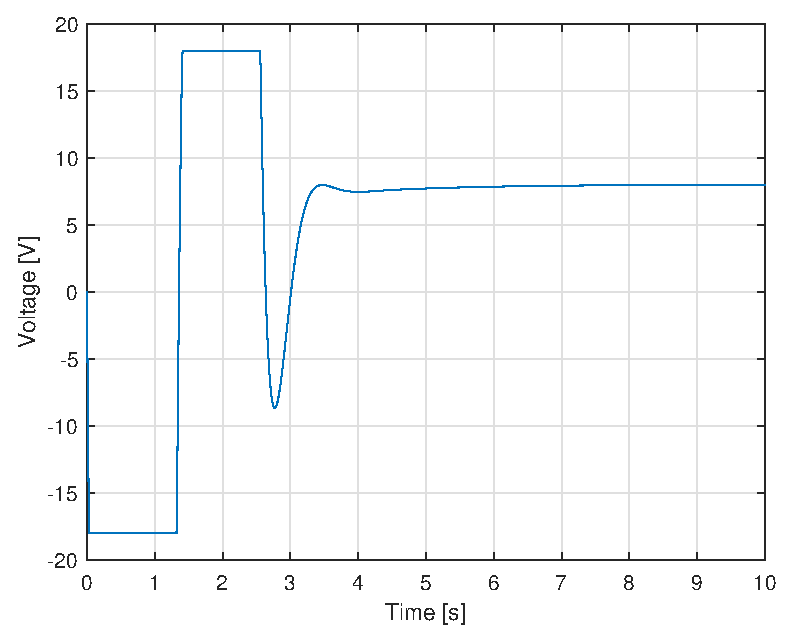
\includegraphics[width=.46\textwidth,keepaspectratio=true]{figs/matlab/LQR/PI_Sim/Pitch_Volt_LQR_Sim.eps}
    \label{fig:Pitch_Volt_LQR_Sim}
    }    
    \subfigure[][]{
    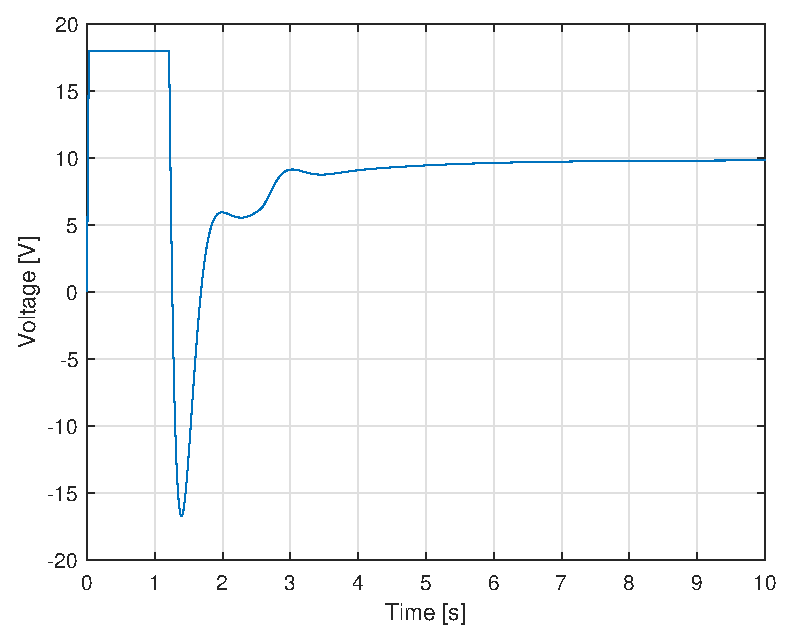
\includegraphics[width=.46\textwidth,keepaspectratio=true]{figs/matlab/LQR/PI_Sim/Yaw_Volt_LQR_Sim.eps}
    \label{fig:Yaw_Volt_LQR_Sim}
    }
    \caption{Simulations for proportional and integral gain calculated by LQR.}
\end{figure}

%----------------------------------------------------------------------
\section{LQG (PI Controller)}
%----------------------------------------------------------------------
\todo[inline]{Insert Block diagram for LQG PI simulation}
%\todo[inline]{Insert results for LQG PI simulation}
\begin{figure}[!htbp]
    \centering
    \subfigure[][]{
    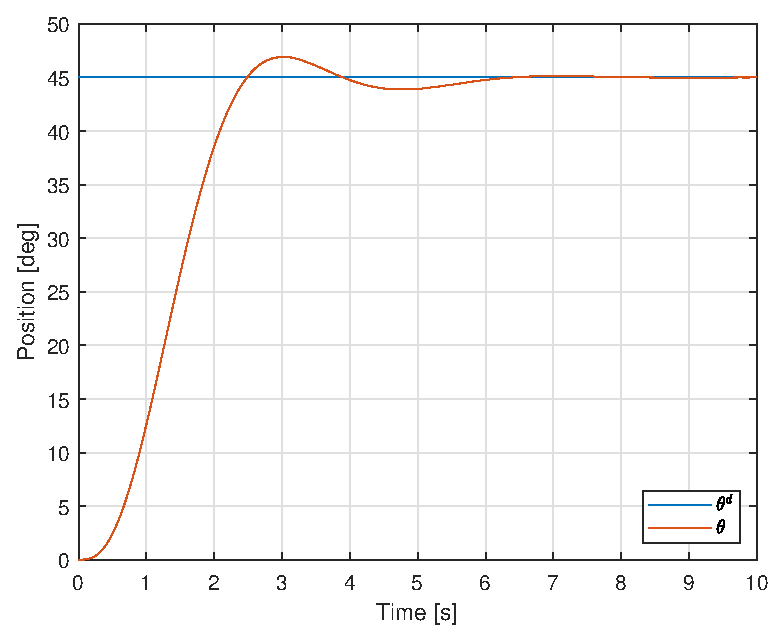
\includegraphics[width=.46\textwidth,keepaspectratio=true]{figs/matlab/LQG/LQG_Sim/Pitch_LQG_Sim.eps}
    \label{fig:Pitch_LQG_Sim}
    }
    \subfigure[][]{
    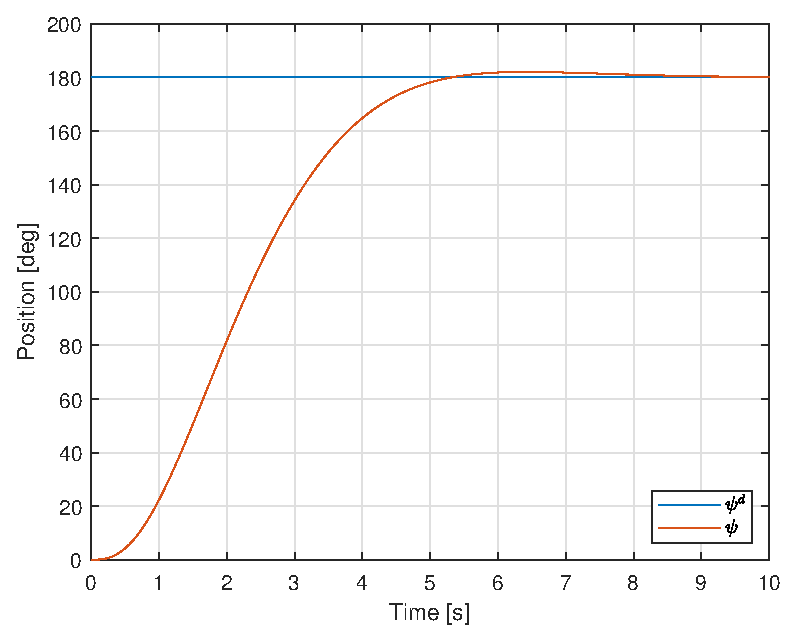
\includegraphics[width=.46\textwidth,keepaspectratio=true]{figs/matlab/LQG/LQG_Sim/Yaw_LQG_Sim.eps}
    \label{fig:Yaw_LQG_Sim}
    }    
    \subfigure[][]{
    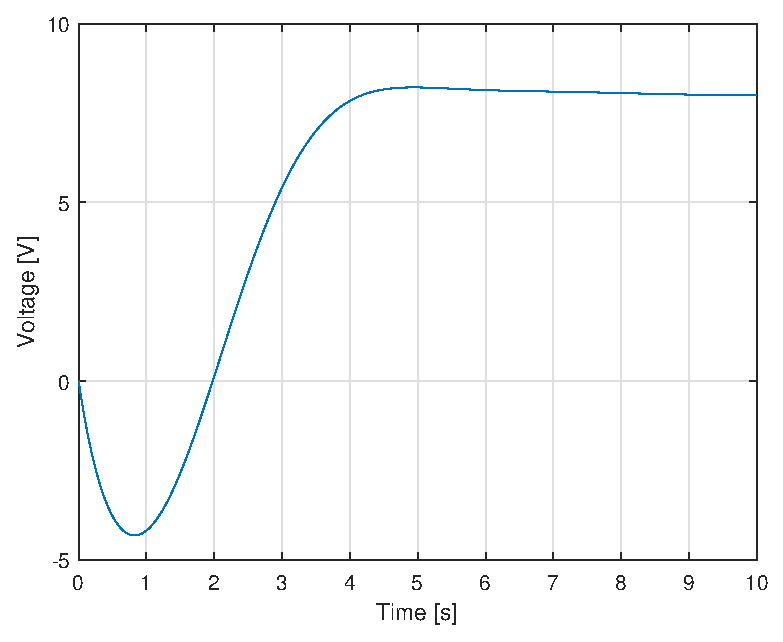
\includegraphics[width=.46\textwidth,keepaspectratio=true]{figs/matlab/LQG/LQG_Sim/Pitch_Volt_LQG_Sim.eps}
    \label{fig:Pitch_Volt_LQG_Sim}
    }    
    \subfigure[][]{
    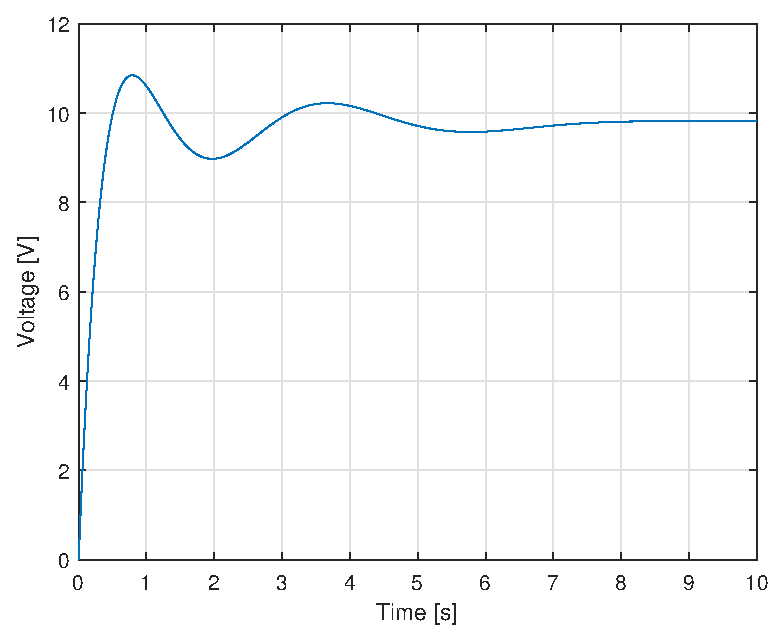
\includegraphics[width=.46\textwidth,keepaspectratio=true]{figs/matlab/LQG/LQG_Sim/Yaw_Volt_LQG_Sim.eps}
    \label{fig:Yaw_Volt_LQG_Sim}
    }
    \caption{Simulations for proportional and integral gain calculated by LQG.}
\end{figure}

%----------------------------------------------------------------------
\section{Conclusions}
%----------------------------------------------------------------------
Note: constant used pitch XXXX degrees, yaw XXXX degrees\\
Note: square used pitch XXXX degrees with period of XXXX, yaw XXXX degrees with period of XXXX\\
Note: sine used pitch XXXX degrees with period of XXXX, yaw XXXX degrees with period of XXXX\\
\begin{table}[!htbp]
    \centering
    \begin{tabular}{l|l|l|l|l|l|l}
        \toprule
        \textbf{} & \textbf{LQR(P)} & \textbf{LQR(PI)} & \textbf{LQG(PI)} \\
        \toprule
        RMSE Pitch Step & ? & ? & ?  \\
        RMSE Yaw Step & ? & ? & ? \\
        RMSE Pitch Square & ? & ? & ? \\
        RMSE Yaw Square & ? & ? & ? \\
        RMSE Pitch Sine & ? & ? & ? \\
        RMSE Yaw Sine & ? & ? & ? \\
        \bottomrule
    \end{tabular}
    \caption{Error Comparison for Simulated Algorithms}
    \label{tab:Simulate_RMSE}
\end{table}
Based on the results XXXX preformed better in the simulations.
%----------------------------------------------------------------------



%%% Local Variables:
%%% mode: latex
%%% TeX-master: "../finalReport"
%%% End:
